\documentclass[a4paper, 12pt, spanish]{article}

\usepackage[paper=a4paper, left=1.5cm, right=1.5cm, bottom=1.5cm, top=3.5cm]{geometry}
\usepackage[spanish, es-noshorthands]{babel}
\usepackage[utf8x]{inputenc}
\usepackage[none]{hyphenat}
\usepackage[colorlinks,citecolor=black,filecolor=black,linkcolor=black,    urlcolor=black]{hyperref}

% Simbolos matemáticos
\usepackage{amsthm}
\usepackage{amsmath}
\usepackage{amsfonts}
\usepackage{amssymb}
\usepackage{algorithm}
\usepackage[noend]{algpseudocode}
\usepackage{algorithmicx}
\usepackage{listings}
\lstset{
    breaklines=true,
    basicstyle=\normalfont\ttfamily,
    frame=single ,
    % basicstyle=\tiny,
    literate=%
        {á}{{\'a}}1
        {í}{{\'i}}1
        {é}{{\'e}}1
        {ú}{{\'u}}1
        {ó}{{\'o}}1
        {ñ}{{\~n}}1
        {Á}{{\'A}}1
        {Í}{{\'I}}1
        {É}{{\'E}}1
        {Ú}{{\'U}}1
        {Ó}{{\'O}}1
        {Ñ}{{\~N}}1
}

% Descoración y gráficos
\usepackage{caratulaV}
\usepackage{graphicx}
\usepackage{fancyhdr}
\usepackage{lastpage}
\usepackage{caption}
\usepackage{subcaption}
\usepackage{multirow}
\usepackage{alltt}
\usepackage{tikz}
\usepackage{color}
\usepackage{gnuplottex}
\usepackage{verbatim}
\usepackage{framed}
\usepackage[font=small,labelfont=bf]{caption}
\usepackage[normalem]{ulem} %para subrayar

% Bibliografía
\usepackage{natbib}

% Del enunciado
\usepackage{a4wide}
\usepackage{amsmath}
\usepackage{amsfonts}
\usepackage{graphicx}
%\usepackage[ruled,vlined]{algorithm2e}

\usepackage{bera}% optional: just to have a nice mono-spaced font
\usepackage{xcolor}

\newcommand{\kknn}{k}
\newcommand{\kpca}{\alpha}
\newcommand{\kkfold}{K}

% Acomodo fancyhdr.
\pagestyle{fancy}
\thispagestyle{fancy}
\addtolength{\headheight}{1pt}
\lhead{Bases de Datos}
\rhead{$2^{\mathrm{do}}$ cuatrimestre de 2015}
\cfoot{\thepage /\pageref*{LastPage}}
\renewcommand{\footrulewidth}{0.4pt}

\floatname{algorithm}{Pseudocódigo}
\algrenewcommand\algorithmicfunction{\textbf{Función}}
\algrenewcommand\algorithmicwhile{\textbf{mientras}}
\algrenewcommand\algorithmicfor{\textbf{para}}
\algrenewcommand\algorithmicforall{\textbf{para cada}}
\algrenewcommand\algorithmicdo{\textbf{hacer:}}
\algrenewcommand\algorithmicif{\textbf{si}}
\algrenewcommand\algorithmicthen{\textbf{entonces:}}
\algrenewcommand\algorithmicelse{\textbf{si no:}}
\algrenewcommand\algorithmicend{\textbf{fin}}
\algrenewcommand\algorithmicreturn{\textbf{devolver}}

\sloppy

\parskip=5pt % 10pt es el tama de fuente

% Pongo en 0 la distancia extra entre itemes.
\let\olditemize\itemize
\def\itemize{\olditemize\itemsep=0pt}

\usepackage{tikz}
%\usepackage{tikz-qtree}


\usetikzlibrary{arrows,backgrounds,calc}

\pgfdeclarelayer{background}
\pgfsetlayers{background,main}

\newcommand{\real}{\mathbb{R}}
\newcommand{\nat}{\mathbb{N}}

\newcommand{\revJ}[1]{{\color{red} #1}}

\newcommand{\convexpath}[2]{
[
    create hullnodes/.code={
        \global\edef\namelist{#1}
        \foreach [count=\counter] \nodename in \namelist {
            \global\edef\numberofnodes{\counter}
            \node at (\nodename) [draw=none,name=hullnode\counter] {};
        }
        \node at (hullnode\numberofnodes) [name=hullnode0,draw=none] {};
        \pgfmathtruncatemacro\lastnumber{\numberofnodes+1}
        \node at (hullnode1) [name=hullnode\lastnumber,draw=none] {};
    },
    create hullnodes
]
($(hullnode1)!#2!-90:(hullnode0)$)
\foreach [
    evaluate=\currentnode as \previousnode using \currentnode-1,
    evaluate=\currentnode as \nextnode using \currentnode+1
    ] \currentnode in {1,...,\numberofnodes} {
-- ($(hullnode\currentnode)!#2!-90:(hullnode\previousnode)$)
  let \p1 = ($(hullnode\currentnode)!#2!-90:(hullnode\previousnode) - (hullnode\currentnode)$),
    \n1 = {atan2(\x1,\y1)},
    \p2 = ($(hullnode\currentnode)!#2!90:(hullnode\nextnode) - (hullnode\currentnode)$),
    \n2 = {atan2(\x2,\y2)},
    \n{delta} = {-Mod(\n1-\n2,360)}
  in
    {arc [start angle=\n1, delta angle=\n{delta}, radius=#2]}
}
-- cycle
}

\newcommand{\todo}[1]{
\textbf{\color{red}{\underline{Nota:} #1}}
}

\newcommand\param[3]{\ensuremath{\mathbf{\textbf{#1}}\,#2\!:} \texttt{#3}}

\let\state\State
\let\while\While
\let\endwhile\EndWhile
\let\endif\EndIf
\let\elseif\ElsIf
\let\for\For
\let\endfor\EndFor
\let\function\Function
\let\endfunction\EndFunction


\newcommand{\degree}{\ensuremath{^\circ}}

\usepackage{caratula}
\materia{Bases de datos}
\submateria{Segundo Cuatrimestre de 2015}
\titulo{Trabajo Práctico II}
% \subtitulo{\emph{Reentrega}}
\fecha{\today}
\integrante{Ignacio Truffat}{837/10}{el\_truffa@hotmail.com}
\integrante{Gaston Rocca}{836/97}{gastonrocca@gmail.com}
\integrante{Agustín Godnic}{689/10}{agustingodnic@gmail.com}
\integrante{Matías Pizzagalli}{257/12}{matipizza@gmail.com}

\begin{document}
\maketitle

\newpage

\tableofcontents

\newpage
\section{Introdución.}
El trabajo práctico esta enfocado en aprender el uso de las diferenctes funcionalidad disponibles en la base de datos MongoDB. Consiste en resolver distintos ejercicios utilizando esta base de datos No relacional. Dentro de las bases No relaciones, Mongo DB es una base orientada a Documentos. Esto quiere decir que en lugar de guardar los datos en registros, guarda los datos en documentos. Estos documentos son almacenados en un formato BSON, que es una representación binaria de JSON.

Una de las diferencias más importantes con respecto a las bases de datos relacionales, es que no es necesario seguir un esquema. Los documentos de una misma colección - concepto similar a una tabla de una base de datos relacional -, pueden tener esquemas diferentes.

En el trabajo vamos a experimentar y desarrollar ejercicios sobre Desnormalización, Map-Reduce y Sharding. También haremos una comparativa con otras bases de datos No Relaciones.

\section{Desnormalización.}
En esta sección del trabajo practico, se trata sobre realizar un diseño orientado a documentos, de un DER provisto por la catedra y utilizando la tecnica de desnormalización. Ademas para tomar como guía del diseño tenemos un par de consultas que debemos poder contestar con nuestro diseño propuesto.

Luego de analizar todas las consultas dadas, llegamos al siguiente diseño:

\begin{lstlisting}
Empleado: {
nroLegajo: int,
nombre: string,
clientes: [{DNI, Nombre, Edad}]
trabajos: [{CodSector, idTarea}]
}

Cliente: {
DNI: int,
nombre: string,
edad: int,
compras: [{CodBarra}]
}

Sector: {
CodSector: int,
Empleados: [ {NroLegajo, idTarea}]
}

Articulo: {
  CobBarras: int,
  nombre: string,
  CodSector: int,
  compradores: [{DNI}]
}

Tarea: {
  idTarea: int,
  Descripcion: string
}

\end{lstlisting}
El diseño se basa en, primero tenemos un tipo de documento por cada entidad del DER y luego le fuimos agregando atributos a cada tipo de documento para ir cumpliendo con las distintas consultas necesarias.

A continuación iremos enfocandonos en cada una de las consultas, explicando que decisiones tomamos en base a esa consulta, permitiendo entender el resultado final del diseño presentado más arriba.


\subsection{Empleados que atendieron clientes mayores de edad.}

Para realizar esta consulta, pensamos un esquema de documento donde embebemos los clientes dentro de los empleados, incluyendo la fecha de cuando fueron atendidos.

\begin{lstlisting}
Empleado: {
  nroLegajo: int,
  nombre: string,
  clientes: [{DNI, Nombre, Edad, Fecha}],
  ...
}
\end{lstlisting}

Luego, para responder la consulta deseada hay que correr:

\begin{lstlisting}
db.empleados.aggregate(
  [
    { $unwind: "$clientes" },
    { $match: {"clientes.Edad": { $gt: 17 } }  },
    { $group: { _id: "$nombre", nombre:{$first:"$nombre" } } },
    { $project : { _id:0, nombre: 1 } }
  ]
)
\end{lstlisting}
\label{consulta-a}

\subsubsection{Ejemplo}

Para insertar registros en la base corremos:

\begin{lstlisting}
db.empleados.insert( {
	nroLegajo: 003,
	nombre: "Ernestino Juanes",
	clientes: [
		{DNI: 40528343,
		Nombre: "Raul Juan Lopez",
		Edad: 14,
		Fecha: "14/03/2015"} ] } )

db.empleados.insert( {
	nroLegajo: 002,
	nombre: "Juan Paez",
	clientes:
	[
		{
		DNI: 30154820,
		Nombre: "Juana Perez",
		Edad: 23,
		Fecha: "20/04/2015"
		},
		{
		DNI: 40528753,
		Nombre: "Raul Lopez",
		Edad: 15,
		Fecha: "23/04/2015"
		}
	] } )

db.empleados.insert( {
	nroLegajo: 001,
	nombre: "Joaquina Paez",
	clientes: [ {
		DNI: 30154820,
		Nombre: "Juan Perez",
		Edad: 25,
		Fecha: "03/04/2015"} ] } )
\end{lstlisting}

Luego, una vez insertados los registros deseados, corremos la consulta mencionada arriba y nos da:

\begin{lstlisting}
{ "nombre" : "Joaquina Paez" }
{ "nombre" : "Juan Paez" }
\end{lstlisting}

\subsection{Artículos mas vendidos.}
Para poder obtener esta información embebimos los DNIs de clientes que compraron cada artículo, dentro del artículo en cuestion. Luego buscamos el artículo con mas compradores y ese es el que nos interesa.

\begin{lstlisting}
Articulo: {
  CobBarras: int,
  nombre: string,
  CodSector: int,
  compradores: [{DNI}]
}
\end{lstlisting}


Entonces, una vez definido el esquema de documento de la coleccion articulos, podemos obtener el maximo mediante la siguiente consulta:
\begin{lstlisting}
db.articulos.aggregate(
  [
    { $unwind : "$Compradores"},
    {$group : { _id: "$CodBarras", CodBarras:{$first:"$CodBarras"},
      Nombre:{$first:"$Nombre"}, totalVendidos: {$sum: 1} } },
    {$sort: {totalVendidos: -1}},
    {$limit : 1},
    {$project : { _id:0,CodBarras: 1, totalVendidos: 1, Nombre: 1}}
  ]
)
\end{lstlisting}

\subsubsection{Ejemplo}
Primero para insertar objetos corremos:
\begin{lstlisting}
db.articulos.insert( { CodBarras: 1303123392, Nombre: "El naufrago",
  CodSector: 2, Compradores: [22222222] } )

db.articulos.insert( { CodBarras: 2303192312,
  Nombre: "El principito", CodSector: 3,
  Compradores: [333333333, 22222222] } )

db.articulos.insert( {CodBarras: 2305110547, Nombre: "La sombra",
 CodSector: 2, Compradores: [ 323333333, 29123654, 28741903 ] } )

\end{lstlisting}

Luego, con los articulos agregados, corremos la consulta y obtenemos:

\begin{lstlisting}
{ "CodBarras" : 2305110547, "Nombre" : "La sombra",
  "totalVendidos" : 3 }
\end{lstlisting}


\subsection{Sectores donde trabajan exactamente 3 empleados.}
Para poder realizar esta consulta, decidimos embeber dentro de sectores una lista con
el numero de legajo de todos los empleados que estan trabajando en el sector y ademas el id de la tarea que
desempeñan en el mismo.

\begin{lstlisting}
Sector: {
CodSector: int,
Empleados: [ {NroLegajo, idTarea}]
}
\end{lstlisting}


Luego tomando como referencia este tipo de documento, realizamos la siguiente consulta:
\begin{lstlisting}
db.sectores.aggregate([{ $unwind : "$Empleados"},
	{$group : {_id: "$CodSector",CodSector:{$first:"$CodSector"},
	totalEmpleados: {$sum: 1}}},{$project : {_id: 0, CodSector: 1,
	totalEmpleados:1}},{$match : {totalEmpleados :3 }} ])
\end{lstlisting}

\subsubsection{Ejemplo}
Primero insertamos algunos sectores con el esquema dado:
\begin{lstlisting}
db.sectores.insert({CodSector: 1, Empleados: [{NroLegajo: 001,
	idTarea: 02},{NroLegajo: 002, idTarea: 03},{NroLegajo: 003,
	idTarea: 01}]})

db.sectores.insert({CodSector: 2,
Empleados: [
	{NroLegajo: 001, idTarea: 01},
	{NroLegajo: 002, idTarea: 07},
	{NroLegajo: 003, idTarea: 01},
	{NroLegajo: 001, idTarea: 02},
	{NroLegajo: 008, idTarea: 12}
	]})

db.sectores.insert({CodSector: 4,
Empleados: [
		{NroLegajo: 007, idTarea: 02},
		{NroLegajo: 003, idTarea: 11}]})
\end{lstlisting}

Luego, ya con los ejemplos insertados, corremos la consulta descripta mas arriba y obtenemos:
\begin{lstlisting}
{ "CodSector" : 1, "totalEmpleados" : 3 }
\end{lstlisting}

\subsection{Empleado que trabaja en más sectores.}
Para poder obtener esta información, primero planteamos el siguiente esquema de documento para la coleccion de empleados, donde tenemos una lista con los sectores donde un empleado trabaja y las tareas que cumple en dicho sector.

\begin{lstlisting}
Empleado: {
nroLegajo: int,
nombre: string,
clientes: [{DNI, Nombre, Edad}]
trabajos: [{CodSector, idTarea}]
}
\end{lstlisting}

Luego, teniendo en cuenta ese esquema de docuemnto, planteamos la siguiente consulta:
\begin{lstlisting}
db.empleados.aggregate([{ $unwind : "$trabajos"},
{$group : {_id: "$nroLegajo",nroLegajo:{$first:"$nroLegajo"},
totalTrabajos: {$sum: 1}}},
{$project : {_id: 0, nroLegajo: 1, totalTrabajos:1}},
{$sort : {totalTrabajos: -1}},
{$limit : 1} ])
\end{lstlisting}

\subsubsection{Ejemplo}

Primero insertamos algunos ejemplos:
\begin{lstlisting}

db.empleados.insert( { nroLegajo: 006, nombre: "Ernestino Juanes",
	clientes: [
		{DNI: 40528343, Nombre: "Raul Juan Lopez", Edad: 14} ] ,
	trabajos: [{CodSector: 07, Tarea: 10}]} )

db.empleados.insert( { nroLegajo: 005, nombre: "Juan Paez",
	clientes: [
		{DNI: 30154820, Nombre: "Juana Perez", Edad: 23},
		{DNI: 40528753, Nombre: "Raul Lopez", Edad: 15} ],
	trabajos: [
		{CodSector: 01, Tarea: 02},
		{CodSector: 04, Tarea: 03},
		{CodSector: 07, Tarea: 09}] } )

db.empleados.insert( { nroLegajo: 004, nombre: "Joaquina Paez",
	clientes: [
		{DNI: 30154820, Nombre: "Juan Perez", Edad: 25} ],
	trabajos: [
		{CodSector: 09, Tarea: 01},
		{CodSector: 03, Tarea: 05}] } )

\end{lstlisting}

Luego si corremos la consulta sobre estos casos obtenemos:

\begin{lstlisting}
{ "nroLegajo" : 5, "totalTrabajos" : 3 }
\end{lstlisting}
Es decir, que el empleado que trabaja en mas sectores es el que tiene numero de Legajo 5 y trabaja en 3 sectores actualmente.

\subsection{Ranking de los clientes con mayor cantidad de compras.}
Para poder obtener el ranking de los clientes segun la cantidad de compras que realizo cada uno, primero
planteamos el siguiente esquema de documentos para la coleccion cliente, donde tenemos una lista con el codigo de barra de todos los productos que compro.

\begin{lstlisting}
Cliente: {
DNI: int,
nombre: string,
edad: int,
compras: [{CodBarra}]
}
\end{lstlisting}


Luego, basandonos en ese esquema de documento, podemos realizar la siguiente consulta para obtener lo deseado:
\begin{lstlisting}
db.clientes.aggregate([{ $unwind: "$compras"},
{$group : {_id: "$DNI",DNI:{$first:"$DNI"},
		nombre:{$first:"$nombre"},totalCompras: {$sum:1}} },
{$project :{ _id:0, DNI:1, nombre:1, totalCompras:1}},
{$sort : {totalCompras : -1}} ] )
\end{lstlisting}

\subsubsection{Ejemplo}
Primero insertamos algunos ejemplos:
\begin{lstlisting}

db.clientes.insert({
	DNI: 32012932,
	nombre: "Guillermo Rodriguez",
	edad: 23,
	compras: [
		{CodBarra: 321},
		{CodBarra: 023},
		{CodBarra: 231},
		{CodBarra: 123}
		]})

db.clientes.insert({
	DNI: 33002654,
	nombre: "Pedro Juanes",
	edad: 28,
	compras: [
		{CodBarra: 023},
		{CodBarra: 231}
		]})

db.clientes.insert({
	DNI: 38165687,
	nombre: "Carolina Hernandez",
	edad: 20,
	compras: [
		{CodBarra: 123}
		]})
\end{lstlisting}

Luego una vez que ya insertamosestos ejemplos, corremos la consulta y obtenemos:
\begin{lstlisting}
{"DNI" : 33002654, "nombre" : "Pedro Juanes", "totalCompras" : 2}
{"DNI" : 32012932, "nombre" : "Guillermo Rodriguez", "totalCompras" : 4}
{"DNI" : 38165687, "nombre" : "Carolina Hernandez", "totalCompras" : 1}
\end{lstlisting}

\subsection{Cantidad de compras realizadas por clientes de misma edad.}
Para poder realizar esta consulta no tuvimos que realizar ninguna modificación, alcanza con el esquema
de documentos que ya mencionamos mas arriba para la coleccion clientes.

Entonces para responder esta consulta podemos hacer:
\begin{lstlisting}
db.clientes.aggregate([{ $unwind: "$compras"},
{$group : {_id: "$edad", edad: {$first:"$edad"},totalCompras:{$sum:1}}},
{$project: {_id: 0, edad: 1, totalCompras: 1}}])
\end{lstlisting}

\subsubsection{Ejemplo}
Ademas de los clientes insertados en el consulta anterior agregamos:

\begin{lstlisting}
db.clientes.insert({
	DNI: 34020253,
	nombre: "Juan Martinez",
	edad: 28,
	compras: [
		{CodBarra: 007},
		{CodBarra: 109},
		{CodBarra: 182}]
		})
\end{lstlisting}

Entonces, corriendo la consulta mencionada mas arriba obtenemos:

\begin{lstlisting}
{ "edad" : 20, "totalCompras" : 1 }
{ "edad" : 28, "totalCompras" : 5 }
{ "edad" : 23, "totalCompras" : 4 }
\end{lstlisting}

\newpage
\section{Map-Reduce.}
Para la resolución de los Map-Reduce tuvimos que cargar diferentes archivos .json. Esto se realizo con las siguientes instrucciones:
\begin{lstlisting}
mongoimport --db DB --collection COLLECTION --file
disposiciones_201*.json --jsonArray

Por ejemplo:
mongoimport --db tp2 --collection disposiciones --file
disposiciones_2014.json --jsonArray
\end{lstlisting}

Luego implementamos las diferentes funciones de map y de reduce en un archivo aparte por claridad y comidad, llamado \texttt{code.js}.
Luego para cargar el código se puede hacer load("code.js") y podremos referenciar a las funciones implementadas en el archivo desde la consola de mongo.

\subsection{Disposiciones de tipo resolución en Abril de 2013.}
\textbf{Map:}
La idea de esta función es, si el documento dado es de tipo resolución y tiene fecha abril del 2013,
emitir("resolucion",cant=1). De esta forma estamos permitiendo que solo emitan los documentos que nos
interesa contar.

\begin{lstlisting}
var map1 = function(){
  var date = this["FechaBOJA"].split('/')
  if(this["Tipo"] == "Resoluciones" && date[1]==4 && date[2]==2013){
    emit(this["Tipo"],1)
  }
}
\end{lstlisting}

\textbf{Reduce:}
La idea del reduce es, sumar los valores que nos pasan, ya sean unos que vienen del map,
o valores parciales que vienen de otro reduce, lo que genera que este reduce sea combinable y se pueda
aplicar varias veces.

\begin{lstlisting}
var reduce1 = function(key,values){
  return Array.sum(values)
}
\end{lstlisting}

Una vez definadas las dos funciones podemos llamar a la función de map-reduce de la forma:
\begin{lstlisting}
db.disposiciones.mapReduce(map1,reduce1,{out: parte2a})
\end{lstlisting}

Lo que nos devuelve una collecion llamada \texttt{parte2a} con nuestra respuesta:

\begin{lstlisting}
> db.parte2a.find()
{ "_id" : "Resoluciones", "value" : 607 }
\end{lstlisting}

\subsection{Disposiciones de cada tipo.}
\textbf{Map:}
La idea de este map es, para cada documento, emitir su tipo y como valor un 1, para poder contar las ocurrencias
de cada tipo de documento.

\begin{lstlisting}
var map2 = function(){
	emit(this["Tipo"],1)
}
\end{lstlisting}

\textbf{Reduce:}
Esta función de reduce al igual que la anterior suma los valores que se le pasan y retorna la suma. De esta forma vamos a terminar
obteniendo la cantidad de ocurrencias de cada tipo posible de documento.
\begin{lstlisting}
var reduce2 = function(key,values){
	return Array.sum(values)
}
\end{lstlisting}

Una vez definadas las dos funciones podemos llamar a la función de map-reduce de la forma:
\begin{lstlisting}
db.disposiciones.mapReduce(map2,reduce2,{out: parte2b})
\end{lstlisting}

Lo que nos devuelve una collecion llamada \texttt{parte2b} con nuestra respuesta:

\begin{lstlisting}
db.parte2b.find()
{ "_id" : "", "value" : 3 }
{ "_id" : "Acuerdos", "value" : 2790 }
{ "_id" : "Acuerdos del Consejo de Gobierno", "value" : 160 }
{ "_id" : "Anuncios", "value" : 17226 }
{ "_id" : "Candidaturas", "value" : 1 }
{ "_id" : "Certificaciones", "value" : 72 }
{ "_id" : "Circular", "value" : 1 }
{ "_id" : "Conflictos Positivos", "value" : 6 }
{ "_id" : "Correcciones de Erratas", "value" : 59 }
{ "_id" : "Correcciones de Errores", "value" : 321 }
{ "_id" : "Correcciones de erratas", "value" : 8 }
{ "_id" : "Correcciones de errores", "value" : 44 }
{ "_id" : "Corrección de errores", "value" : 1 }
{ "_id" : "Correción de errores", "value" : 1 }
{ "_id" : "Cuestiones de Inconstitucionalidad", "value" : 1 }
{ "_id" : "Decretos", "value" : 828 }
{ "_id" : "Decretos Legislativos", "value" : 5 }
{ "_id" : "Decretos del Presidente", "value" : 13 }
{ "_id" : "Decretos-leyes", "value" : 15 }
{ "_id" : "Edictos", "value" : 3223 }
{ "_id" : "Instrucciones", "value" : 2 }
{ "_id" : "Leyes", "value" : 12 }
{ "_id" : "Notificaciones", "value" : 768 }
{ "_id" : "Orden", "value" : 4 }
{ "_id" : "Otros", "value" : 45 }
{ "_id" : "Reales Decretos", "value" : 5 }
{ "_id" : "Recursos de Inconstitucionalidad", "value" : 7 }
{ "_id" : "Requisitorias", "value" : 2 }
{ "_id" : "Resoluciones", "value" : 13956 }
{ "_id" : "Órdenes", "value" : 2061 }
{ "_id" : "Órdenes de Comision Delegada", "value" : 2 }
\end{lstlisting}

\subsection{Fecha mas citada.}

\textbf{Map:}
La idea de esta función es primero, parsear las fechas que encontramos en el documento exceptuando las que encontremos en la descripción (es decir la fechaBOJA y la fechaDisposicion) y hacer que sus formatos sean compatibles entre si.
Luego una vez obtenidas las fechas, emitimos una vez por cada fecha, tomando como clave la fecha con formato compatible y como valor un 1.
De esta forma podremos contar las ocurrencias de cada una de las fechas que aparecen citadas.

\begin{lstlisting}
var map3 = function(){
	var date = (this["FechaDisposicion"].split('T'))[0].
		split('-').reverse().join('/');
	emit(date,1);
	emit(this["FechaBOJA"],1);
}
\end{lstlisting}
\textbf{Reduce:}
La idea de este reduce al igual que los anteriores es simplemente sumar los valores que recibe.

\begin{lstlisting}
var reduce3 = function(key,values){
	return Array.sum(values)
}
\end{lstlisting}
Una vez definadas las dos funciones podemos llamar a la función de map-reduce de la forma:

\begin{lstlisting}
db.disposiciones.mapReduce(map3,reduce3,{out: parte2c})
\end{lstlisting}

Una vez ejecutado el mapReduce tendremos en la coleccion llamada \texttt{parte2c} todas las fechas citadas con sus respectivas cantidades de ocurrencias. Luego una vez tenemos esa informacion, lo unico que nos falta hacer es ordenar esta coleccion por cantidad de ocurrencias de manera descendente y quedarnos con el primer elemento, es decir:

\begin{lstlisting}
db.parte2c.find().sort({value : -1}).limit(1)
{ "_id" : "12/06/2012", "value" : 364 }
\end{lstlisting}

\subsection{Mayor cantidad de páginas por cada tipo.}

\textbf{Map:}
Lo que realiza la funcion map es, primero calcula la cantidad de paginas q ocupa el documento dado y luego emite su tipo como clave y la cantidad de paginas calculada como valor. Esto nos va a permitir calcular para cada tipo de documento, su máxima cantidad de paginas utilizada.

\begin{lstlisting}
var map4 = function(){
	var cantPags = this["PaginaFinal"] - this["PaginaInicial"] + 1
	emit(this["Tipo"],cantPags)
}
\end{lstlisting}
\textbf{Reduce:}
Esta función busca el maximo entre todos los valores que le pasan y lo devuelve, al emitir lo mismo que recibe este reduce tambien
es combinable y se puede aplicar mas de una vez.
\begin{lstlisting}
var reduce4 = function(key,values){
	var cantPagsMax = 0;
	for (var i=0; i < values.length; i++){
		if(values[i] > cantPagsMax){
			cantPagsMax = values[i];
		}
	}
	return(cantPagsMax);
}
\end{lstlisting}

Una vez definadas las dos funciones podemos llamar a la función de map-reduce de la forma:

\begin{lstlisting}
db.disposiciones.mapReduce(map4,reduce4,{out: parte2d})
\end{lstlisting}

Luego, en la coleccion \texttt{parte2d} encontraremos nuestra respuesta, es decir para cada tipo de documento la cantidad máxima de paginas utilizada por algun documento suyo.

\begin{lstlisting}
> db.parte2d.find()
{ "_id" : "", "value" : 16 }
{ "_id" : "Acuerdos", "value" : 12 }
{ "_id" : "Acuerdos del Consejo de Gobierno", "value" : 83 }
{ "_id" : "Anuncios", "value" : 393 }
{ "_id" : "Candidaturas", "value" : 68 }
{ "_id" : "Certificaciones", "value" : 47 }
{ "_id" : "Circular", "value" : 3 }
{ "_id" : "Conflictos Positivos", "value" : 1 }
{ "_id" : "Correcciones de Erratas", "value" : 174 }
{ "_id" : "Correcciones de Errores", "value" : 99 }
{ "_id" : "Correcciones de erratas", "value" : 10 }
{ "_id" : "Correcciones de errores", "value" : 5 }
{ "_id" : "Corrección de errores", "value" : 1 }
{ "_id" : "Correción de errores", "value" : 1 }
{ "_id" : "Cuestiones de Inconstitucionalidad", "value" : 1 }
{ "_id" : "Decretos", "value" : 492 }
{ "_id" : "Decretos Legislativos", "value" : 37 }
{ "_id" : "Decretos del Presidente", "value" : 3 }
{ "_id" : "Decretos-leyes", "value" : 139 }
{ "_id" : "Edictos", "value" : 48 }
{ "_id" : "Instrucciones", "value" : 3 }
{ "_id" : "Leyes", "value" : 194 }
{ "_id" : "Notificaciones", "value" : 11 }
{ "_id" : "Orden", "value" : 7 }
{ "_id" : "Otros", "value" : 65 }
{ "_id" : "Reales Decretos", "value" : 1 }
{ "_id" : "Recursos de Inconstitucionalidad", "value" : 1 }
{ "_id" : "Requisitorias", "value" : 1 }
{ "_id" : "Resoluciones", "value" : 454 }
{ "_id" : "Órdenes", "value" : 634 }
{ "_id" : "Órdenes de Comision Delegada", "value" : 2 }
\end{lstlisting}

\newpage
\section{Sharding.}

MongoDB utiliza esta técnica para gestionar la carga de los servidores. Distribuye los datos entre distintos shards (conjuntos de servidores que almacenan parte de los datos), para que la carga a la hora de realizar consultas e inserciones se reparta.

\subsection{Pasos para la generación de resultados:}

Levantamos cinco shards siguiendo las instrucciones del archivo tutorial\_sharding.txt.

Luego creamos un indice simple sobre el atributo codigo\_postal.

Luego importamos el código de insert\_data.js donde tenemos
funciones que nos permiten ingresar datos de a 20k y pedir las estadísticas.
Finalmente, nos guardamos las estadísticas en archivos .txt. Los mismos se encuentran en
la carpeta mediciones.

\textbf{Generacion de Datos (insert\_data.js)}
\begin{lstlisting}
var insertData = function(dbName, colName, num) 
{
	var col = db.getSiblingDB(dbName).getCollection(colName);
	
	for (i = 0; i < num; i++) 
	{
		x = Math.floor(Math.random() * 1000000);
		doc = 
		{
			nombre: 'Martin Juarez',
			password: 'asdasd' ,
			codigo_postal: x,
			genero: 'masculino',
			edad: 29,
			fecha_creacion: '30/02/2015'
		}
		col.insert(doc);
	}
	
	print(col.count());
	print(col.getShardDistribution());
	print("##############################################");
}

var insertDataTotal = function(dbName, colName, step, total) 
{
	var col = db.getSiblingDB(dbName).getCollection(colName);
	
	while(col.count() < total)
	{
		for (i = 0; i < step; i++) 
		{
			x = Math.floor(Math.random() * 1000000);
			doc = {
				nombre: 'Martin Juarez',
				password: 'asdasd' ,
				codigo_postal: x,
				genero: 'masculino',
				edad: 29,
				fecha_creacion: '30/02/2015'
			}
			col.insert(doc);
		}
		
		print(col.count());
		print(col.getShardDistribution());
		print("##########################################");
	}
}
\end{lstlisting}
\subsection{Resultados}
\begin{figure}[H]
\centering
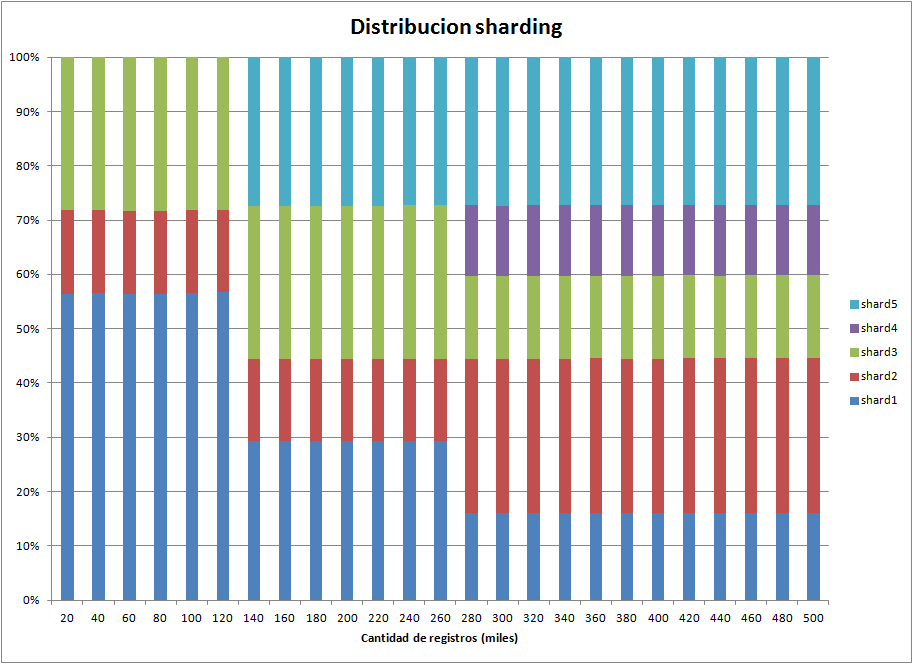
\includegraphics[width=165mm]{../mediciones/sharding_simple.png}
\caption{Porcentaje de distribucion entre los shards usando un
indice simple en base al codigo postal.}
\end{figure}
El primer resultado obtenido corresponde a la distribución de carga con el indice simple sobre código postal. En este caso la distribución no es uniforme, al comienzo gran parte de la carga se la lleva el Shard1 y no intervienen los Shard4 y Shard5. Esto es asi, porque se van llenando los primeros Shards, cuando esto ocurre luego de insertar unos 140.000 registros, vemos que comienzan a distribuirse en el Shard5, y el peso del Shard1 baja a un 30\%.
Al insertar unos 280.000 registros, y de ahí en adelante, el Shard4 comienza a registrar carga. Y en general, todos los shards tienen documentos. 

Ahora veremos como influye la generación de un indice Hash en base al \_id.
\begin{figure}[H]
\centering
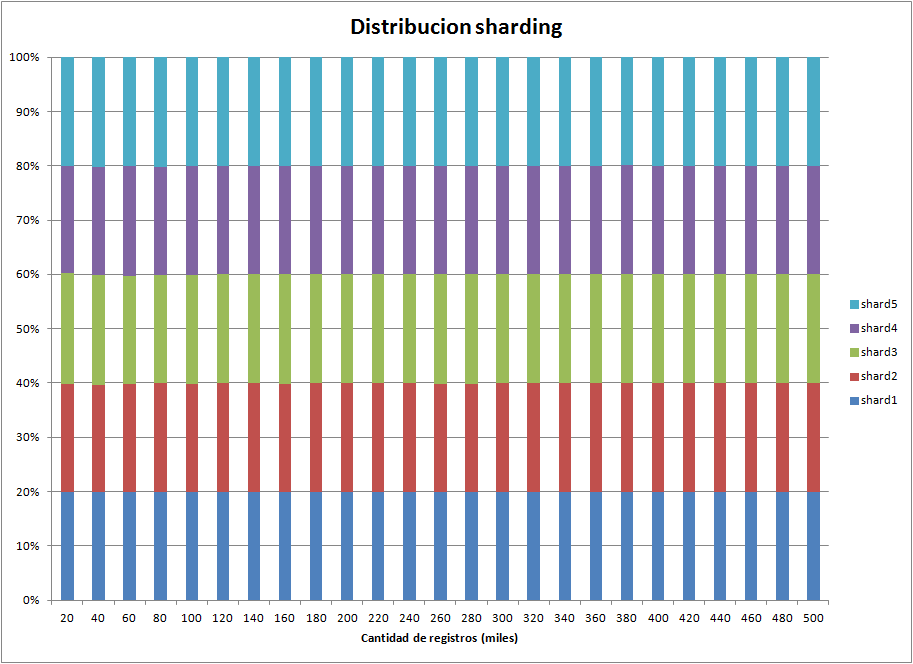
\includegraphics[width=165mm]{../mediciones/sharding_hashed.png}
\caption{Porcentaje de distribución entre los shards usando un
indice hasheado en base al \_id}
\end{figure}

En este caso, el indice hash hace que la distribución de los documentos sea muy equitativa entre los distintos Shards. Desde el comienzo de la carga de registros, se puede ver que todos los Shards tienen aproximadamente un 20 \% de carga.

Esto nos hace reflexionar sobre la importancia de la elección de los indices y su influencia en la distribución de la carga.

Los atributos deben poseer ciertas características para ser candidatos a claves en un esquema de Sharding. La distribución de sus valores debe ser lo mas equiprobable posible dentro de los distintos Shards. Por ejemplo, si tomamos Edad como clave en modelo de pirámide poblacional de un país, es probable que la distribución este mas concentrada en algunos Shards y no en otros. Los shards que contengas las edades mayores a 60 o 70 años tendrán pocos documentos. Dependiendo el país que tomemos, encontraremos mayor distribución de documentos en edades medias o en edades menores a 20 años.

Lo importante es encontrar claves dentro del modelo que reflejen una distribución equiprobable(o similar) y con esto, garantizar un balance de carga entre los diferentes Shards.




\newpage
\section{Otras base de datos NoSql.}


Elegimos bases de datos key-value, el caso particular que analizamos es redis.
Redis permite el uso de namespaces (tener varios "diccionarios", la terminología de redis para esto sería "multiple databases"), lo cual hace el diseño más prolijo y simple.

Usar map-reduce en redis no es algo built-in ni estandar, pero investigamos y es posible, por
    ejemplo, integrarlo con Hadoop.

\begin{description}
\item[1a] En redis hay un comando SCAN que permite iterar las claves.
        Con esto podemos iterar un diccionario de empleados, donde en cada
            value hay una lista de datos de cada cliente que atendió
            ( empleado -> [cliente] ).
        Entonces se puede iterar las claves una por una y quedarse con las que
            tienen algun cliente mayor de edad.
\item[1b]
        Usando SCAN se puede iterar las claves de un diccionario
        articulos -> [ventas]. Mediante codigo se buscan las claves que tengan
        |ventas| maximo.
\item[1c]
        Idem usando SCAN. Si tenemos un diccionario sector -> [empleados], es cuestion
            de iterar y mediante código buscar cuando |empleados|==3

\item[1d]
        Un diccionario empleado -> [sectores]. Idem 1c usando SCAN.

\item[1e]
        Diccionario cliente  -> [compras]. Idem 1c, pero ordenando mediante |compras|.

\item[1f]
        Esta consulta ya es un poco más compleja, hay varios enfoques posibles.
        Uno es mantener las cosas simples y directamente usar un diccionario
            edad -> cantidadDeCompras. Por ser tan específico, es un diccionario
            que sólo sirve para esta consulta, con lo cual estamos agregando
            un costo de mantenimiento extra a la DB sólo por una query.
        Otra opción es valerse de map reduce y usar alguno de los otros diccionarios,
            como el de 1a. Como ventaja, la consulta es simple y no hace falta crear un diccionario extra
            solo por esta consulta.

\item[mapReduce]
    Asumimos que se crea un id único para las disposiciones, podría ser un hash de sus datos o
        la combinación (numeroBoja, paginaInicial, PaginaFinal) que asumimos que identifica
        univocamente a la disposicion. Entonces se tiene un diccionario id -> disposicion,
        sobre el cual podríamos correr todas las consultas por map reduce.

    Dichas resoluciones por map-reduce son prácticamente iguales a las versiones hechas en mongodb
        ya que la entrada de la función map es practicamente la misma.

\end{description}

%Parte 3:
    %TODO: primero habría que hacerlo en mongodb jaja.



\newpage
\section{Conclusiones.}
En cuanto a la tecnica map-reduce, nos dimos cuenta que es una herramienta muy útil para realizar consultas que necesiten de agrupamientos o de agregasiones, ya que su forma de funcionar hace que la solución resulte muy intuitiva. Además resulta interesante para realizar procesamiento sobre bases de datos muy voluminosas ya que permite dividir esta en partes y realizar procesos en simultaneo y distribuidos.

El sharding es una herramienta muy útil para balancear la carga de datos entre servidores. MongoDB nos proporciona una forma sencilla de hacerlo, pero que hay que configurar correctamente. La elección de la clave por la que se realizará el sharding (shard key) es muy importante. Esta elección no se puede cambiar una vez se ha establecido.

Los índices son un punto importante a la hora de realizar consultas contra una base de datos MongoDB. Una mala gestión de los índices puede derivar en un rendimiento pobre, por lo que deberemos ser conscientes del tipo de consultas que se realizan a la base de datos. Sabiendo qué campos se utilizan para filtrar y cuáles suelen ser los devueltos en las consultas, seremos capaces de crear los índices necesarios para que nuestra base de datos se comporte correctamente.

Uno de los aspectos que vimos en la sección en la que investigamos sobre Redis y bases de datos key-value, es que al agregar muchas consultas empieza a necesitarse muchos diccionarios (namespaces) perjudicando asi el diseño y aumentando el costo de mantenimiento de la base. Con lo cual el uso de este tipo de bases de datos es mas idoneo para cuando se tienen pocas consultas para las cuales se necesita buena performance.


\end{document}
